\chapter{Background and Literature Review} \label{chap:ch2}

\section{Quality of Experience and Methodologies for Video Quality Assessment}  

\subsection{Quality of Experience (QoE): A Holistic Framework}  
Quality of Experience (QoE) has emerged as a multidimensional framework for evaluating multimedia services, 
which encompasses technical, perceptual, and contextual factors that collectively define end-user satisfaction ~\cite{itu2012recommendation}. 
Unlike traditional Quality of Service (QoS) metrics, which focus solely on network performance (e.g., latency, packet loss), 
QoE integrates human-centric elements such as user expectations, emotional engagement, and situational context ~\cite{brunnstrom2013qualinet}. 
Within this framework, video quality remains a critical determinant of QoE, as visual fidelity directly impacts viewer retention and satisfaction, 
particularly in applications such as streaming services, video conferencing, and immersive media ~\cite{wang2004ssim}.

\subsection{Video Quality Assessment Paradigms}  
Video Quality Assessment (VQA) methodologies are broadly categorized into two paradigms, each addressing distinct requirements and constraints.  

\begin{itemize}  
    \item \textbf{Subjective Assessment:} Regarded as the "ground truth" for perceptual quality, subjective evaluation relies on human observers to rate video quality using standardized protocols such as the Absolute Category Rating (ACR) or Double-Stimulus Impairment Scale (DSIS) defined in ITU-R BT.500 \cite{itu2012recommendation}. These methods yield metrics like the Mean Opinion Score (MOS), which quantifies perceived quality on a standardized scale (e.g., 1–5). However, subjective assessments are labor-intensive, costly, and impractical for real-time systems due to their reliance on controlled environments and large participant cohorts.  

    \item \textbf{Objective Assessment:} Objective methods employ computational models to predict quality automatically, enabling scalable and real-time evaluations. These approaches are further classified into:  
    \begin{itemize}  
        \item \textbf{Full-Reference (FR):} Compares distorted content against a pristine reference (e.g., PSNR, SSIM).  
        \item \textbf{Reduced-Reference (RR):} Uses partial reference data (e.g., feature vectors).  
        \item \textbf{No-Reference (NR):} Operates without reference signals, ideal for live-streaming and broadcast monitoring.  
    \end{itemize}  
\end{itemize}  

\subsection{The Case for No-Reference Video Quality Assessment}  
This dissertation focuses on \textbf{No-Reference (NR) VQA}, a critical enabler for real-time quality monitoring in applications where reference content is unavailable or impractical to obtain (e.g., live sports streaming, user-generated content platforms). NR methods infer quality directly from distorted signals using machine learning, deep neural networks, or perceptual models, balancing computational efficiency with prediction accuracy \cite{min2024perceptual}. The absence of reference data, however, introduces challenges such as:  
\begin{itemize}  
    \item \textbf{Content Dependency:} Algorithms must generalize across diverse video genres (e.g., animations, natural scenes).  
    \item \textbf{Distortion Complexity:} Real-world distortions (e.g., compression artifacts, motion blur) often coexist, complicating feature extraction.  
    \item \textbf{HVS Alignment:} Models must mimic human perception to ensure meaningful quality scores \cite{wang2004ssim}.  
\end{itemize}  

\subsection{Foundational Objective Metrics}  
\label{subsec:metrics}  
Objective metrics serve as the backbone for developing and benchmarking NR models. Two widely adopted FR metrics are:  

\subsubsection{Peak Signal-to-Noise Ratio (PSNR)}  
\begin{equation}  
\text{PSNR} = 10 \cdot \log_{10}\left(\frac{\text{MAX}^2}{\text{MSE}}\right)  
\label{eq:psnr}  
\end{equation}  
PSNR quantifies the logarithmic ratio between the maximum pixel value ($\text{MAX}$, typically 255 for 8-bit images) and the Mean Squared Error ($\text{MSE}$) between reference ($x$) and distorted ($y$) frames:  
\[  
\text{MSE} = \frac{1}{N} \sum_{i=1}^{N} (x_i - y_i)^2,  
\]  
where $N$ is the total number of pixels. Despite its simplicity, PSNR correlates poorly with human perception, as it ignores structural distortions and contextual relevance \cite{huynh2012scope}.  

\subsubsection{Structural Similarity Index (SSIM)}  
\begin{equation}  
\text{SSIM}(x, y) = \frac{(2 \mu_x \mu_y + C_1)(2 \sigma_{xy} + C_2)}{(\mu_x^2 + \mu_y^2 + C_1)(\sigma_x^2 + \sigma_y^2 + C_2)}  
\label{eq:ssim}  
\end{equation}  
SSIM, introduced by Wang et al. \cite{wang2004ssim}, addresses PSNR's limitations by modeling three perceptual components:  
\begin{itemize}  
    \item \textbf{Luminance ($\mu_x, \mu_y$):} Mean intensity, reflecting brightness similarity.  
    \item \textbf{Contrast ($\sigma_x, \sigma_y$):} Standard deviation, capturing texture and edge variations.  
    \item \textbf{Structure ($\sigma_{xy}$):} Covariance, assessing spatial correlation between $x$ and $y$.  
\end{itemize}  
The constants $C_1$ and $C_2$ stabilize the computations in regions with low intensity. SSIM ranges from $-1$ (dissimilar) to $1$ (identical), with higher values indicating superior quality. Extensions like 3D-SSIM \cite{zeng2012_3dssim} enhance its utility for video by incorporating temporal dynamics, while multiscale implementations (MS-SSIM) improve robustness to resolution changes \cite{wang2003multiscale}.  

\subsection{Evolution to Data-Driven NR VQA}  
The limitations of hand-made metrics such as PSNR and SSIM have led to the adoption of data-driven NR models. Modern approaches leverage:  
\begin{itemize}  
    \item \textbf{Deep Neural Networks (DNNs):} Architectures such as ResNet \cite{he2016deep} and Vision Transformers (ViTs) \cite{dosovitskiy2020image} extract spatiotemporal features directly from distorted videos.  
    \item \textbf{Hybrid Frameworks:} Combine traditional metrics with machine learning (e.g., MDVSFA \cite{li2023unified} uses ResNet-50 for feature extraction).  
    \item \textbf{End-to-End Optimization:} Models like FastVQA \cite{wu2022fastvqa} prioritize computational efficiency for real-time applications.  
\end{itemize}  
These advances underscore the shift from heuristic models to adaptive, learning-based systems capable of addressing the complexity of in-the-wild video distortions \cite{min2024perceptual}. 

\subsection{Media Production Workflows and the Role of QoE Assessment}

Professional media production and delivery constitute a complex, multi-stage workflow involving numerous processes, each contributing distinctly to the end-user Quality of Experience (QoE). This pipeline begins with content acquisition, where audiovisual data is captured using high-resolution cameras and initial encoding takes place. The raw footage typically undergoes intensive post-production stages including editing, color grading, audio mixing, and the integration of visual effects. These processes substantially influence perceived quality by shaping aesthetic aspects, narrative coherence, and audiovisual clarity.

Following post-production, the content is prepared for distribution through encoding and transcoding stages. Here, compression algorithms are applied to ensure optimal delivery across diverse platforms—ranging from traditional broadcast to modern adaptive streaming protocols (e.g., MPEG-DASH, HLS). Compression and transcoding introduce artifacts such as blockiness, blurring, and temporal inconsistencies, each affecting QoE differently based on user device capabilities, network conditions, and content type.

Distribution itself, particularly via streaming, introduces another critical dimension to quality assessment. Adaptive bitrate streaming mechanisms dynamically modify video quality according to real-time network conditions and playback buffer states. This adaptation aims to minimize interruptions, stalls, and quality fluctuations, all of which directly impact user experience. Accurate QoE estimation at this stage becomes essential for making informed streaming decisions, as it balances resource efficiency (bandwidth consumption, infrastructure costs) against the perceived quality delivered to end-users.

Finally, the playback environment (end-user devices and software) also imposes constraints affecting perceived quality. Variations in screen resolution, decoding capabilities, and viewing conditions introduce additional complexities into the QoE assessment process.

Within this comprehensive workflow, the accurate measurement and prediction of QoE emerges as a critical task. Traditional metrics such as Peak Signal-to-Noise Ratio (PSNR) and Structural Similarity Index (SSIM) are insufficient for capturing the nuances of human perception under real-world viewing conditions and dynamic streaming impairments. To overcome these limitations, advanced no-reference deep learning-based QoE models, capable of assessing video quality continuously and perceptually, are increasingly adopted.

The QoE inference mechanism developed in this dissertation specifically addresses these industry needs. Positioned at the distribution or playback stages—particularly at the CDN edge or client-side—this real-time system leverages a dual-stage attention neural network architecture, efficiently implemented in Rust, to provide continuous, accurate QoE predictions. Such real-time perceptual quality scores enable streaming providers to dynamically adjust bitrate, detect and preempt service degradation events, and enhance overall viewer satisfaction. Thus, this work bridges theoretical perceptual modeling with practical deployment considerations, facilitating QoE-driven optimization across professional media pipelines.

\section{State-of-the-Art Video Quality Assessment Algorithms}\label{sec:se21}

As summarized by a recent survey~\cite{min2024perceptual}, several objective No-Reference Video Quality Assessment (NR VQA) algorithms have demonstrated exceptional performance on commonly used databases. These state-of-the-art algorithms are predominantly based on frameworks built using Deep Neural Networks (DNN), which form the central focus of this study. 

One of these high-performing algorithms, proposed by Wu, Chen, Hou, et al., and referred to as FastVQA~\cite{wu2022fastvqa}, utilizes a unique framework designed for efficient end-to-end video quality assessment. The framework implements fragment sampling to extract critical spatiotemporal features from video sequences, reducing computational complexity while maintaining high-quality predictions. By leveraging an end-to-end training architecture, FastVQA is particularly well-suited for real-time video quality assessment applications, where speed and accuracy are critical. The framework described for this algorithm is highlighted in Figure ~\ref{fig:framework1} and can be described by the two following aspects, which are Grid Mini-patch Sampling (GMS) and the Fragment Attention Network (FANet).

\begin{figure}
    \centering
    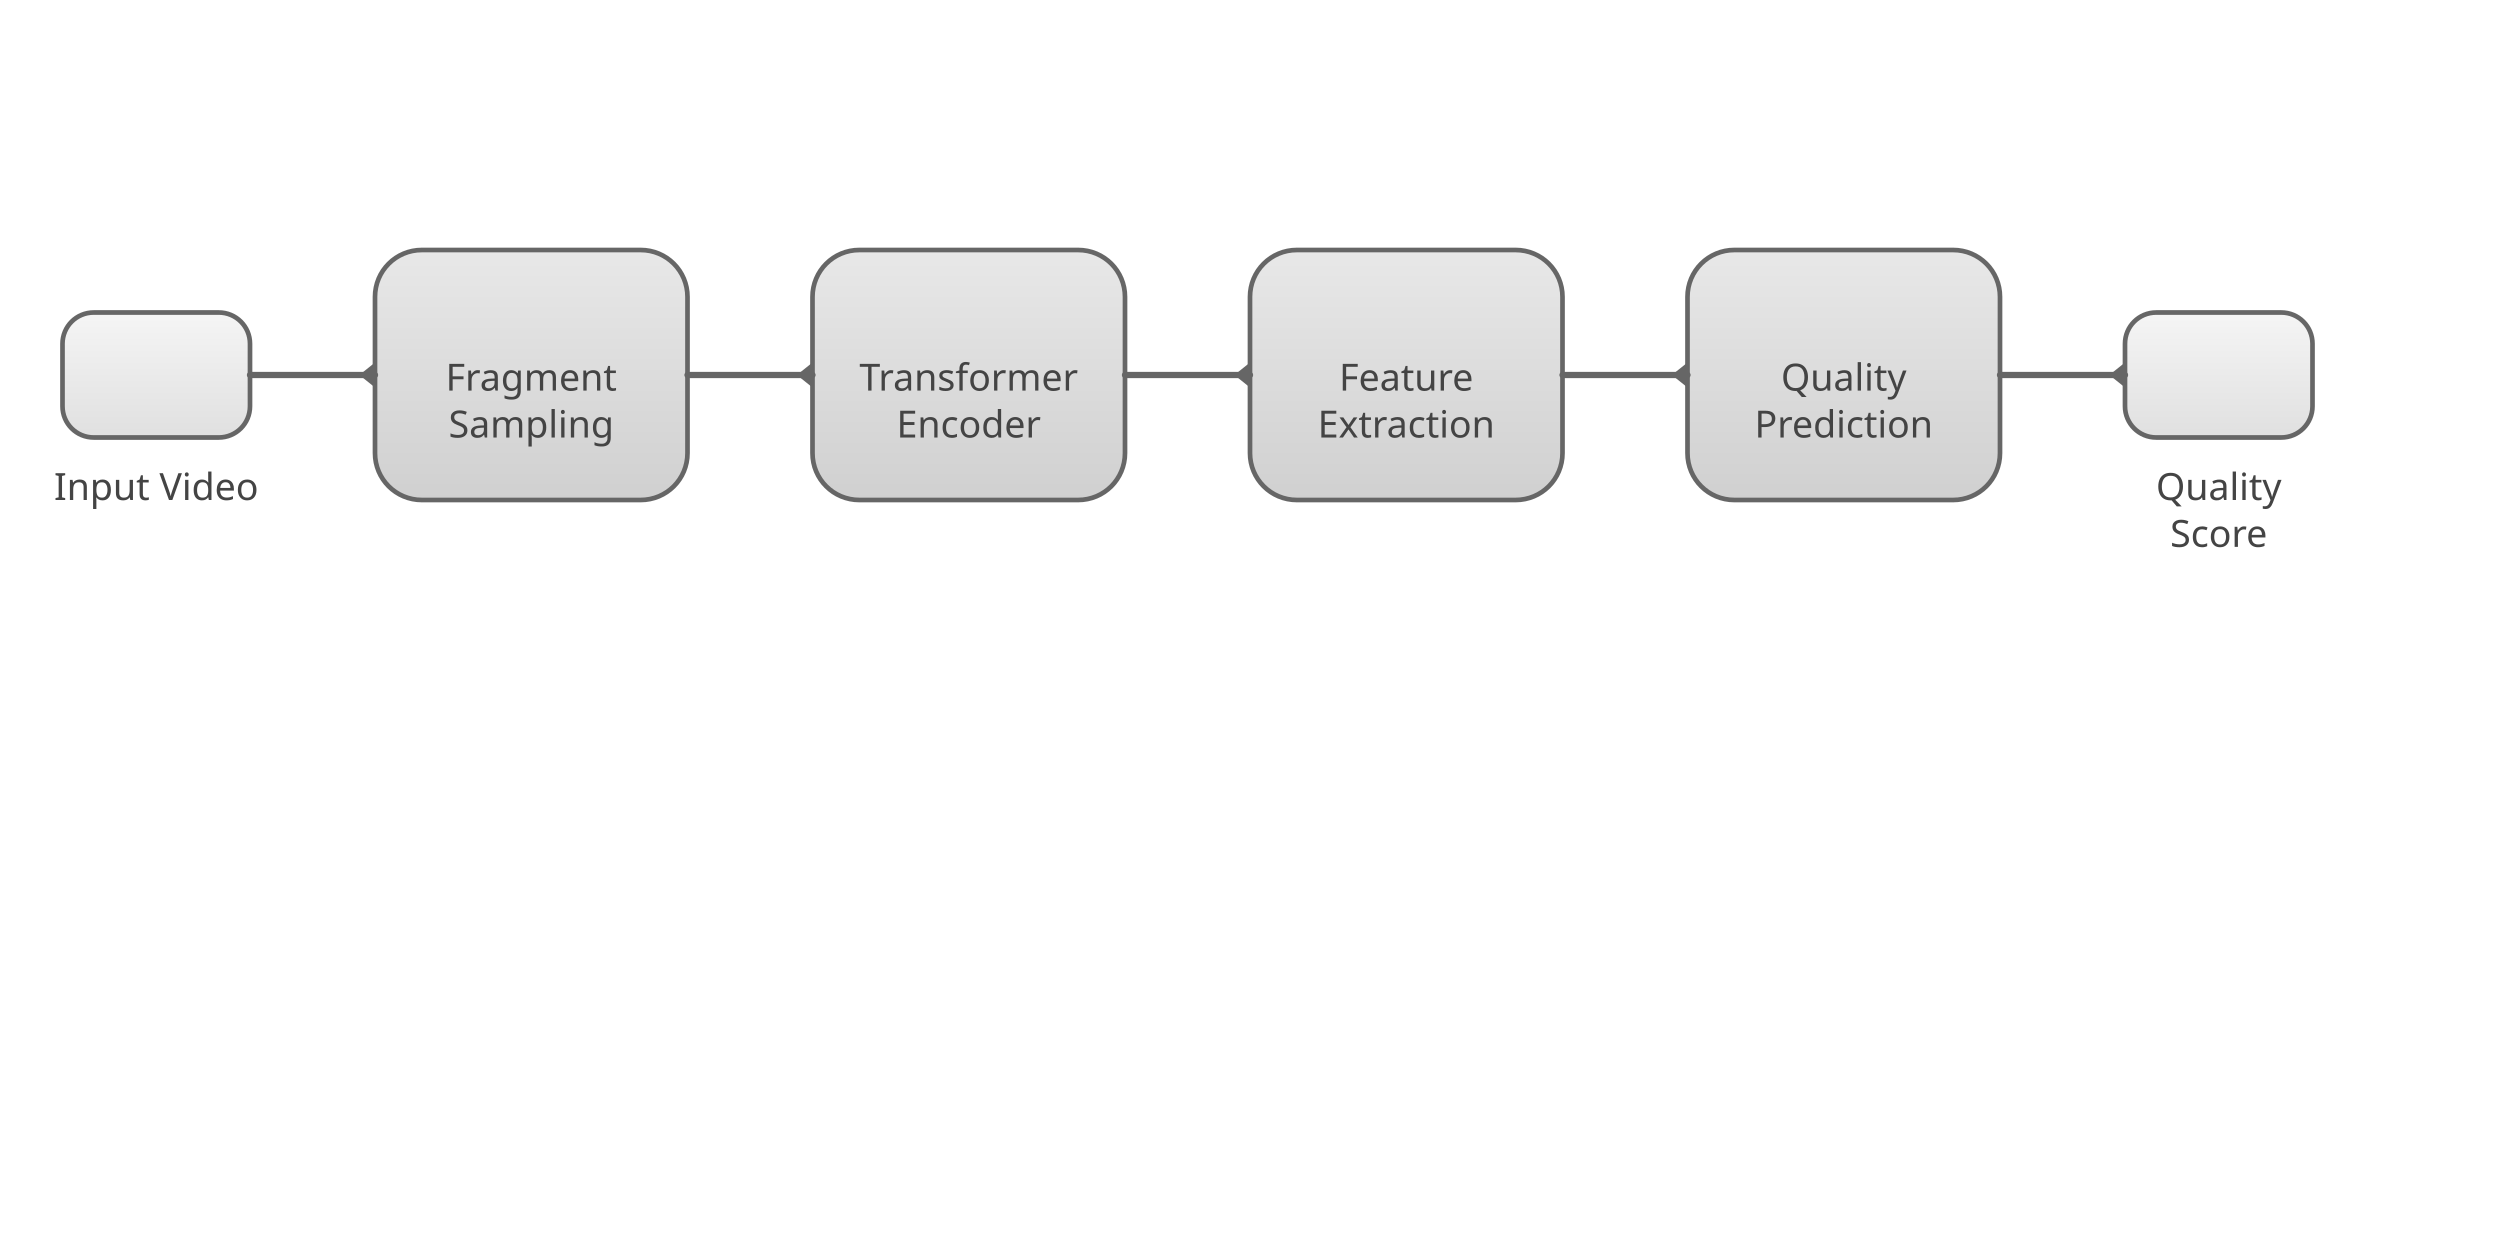
\includegraphics[width=0.9\textwidth]{figures/fast-vqa-framework-3.png}
    \caption{Framework of the algorithm proposed by Wu, Chen, Hou, et al.~\cite{wu2022fastvqa}}
    \label{fig:framework1}
\end{figure}

Grid Mini-patch Sampling (GMS) is a technique designed to capture both global and local video quality features while maintaining efficiency. The process begins by dividing video frames into a uniform grid, preserving global quality. Each frame is divided into smaller grids \(G_f \times G_f\), ensuring that every region of the frame is uniformly assessed, as shown in Equation~\ref{eq:gms_grid}. This grid partition ensures that quality is evaluated in all regions, providing a thorough and balanced analysis.

\begin{equation}
G_f = \frac{\text{Frame Width}}{\text{Grid Size}}, \quad G_f = \frac{\text{Frame Height}}{\text{Grid Size}}
\label{eq:gms_grid}
\end{equation}

To preserve local video quality, raw resolution mini-patches are selected from each grid without resizing, maintaining the original texture of the frame. This helps to retain fine-grained details, such as blurring, noise, and artifacts, which are essential for accurate Video Quality Assessment (VQA). The patches, denoted by $MP_{i,j_t}$, are sampled randomly from each grid, ensuring that the local textural information is captured effectively.

For temporal quality, the sampling process guarantees that patches from different frames are aligned temporally, ensuring consistency across frames. This alignment ensures that the raw temporal variations, which influence the video quality, are retained throughout the entire video sequence. The temporal alignment is enforced by applying the same sampling operation to corresponding regions of each frame, as stated in Equation~\ref{eq:temporal_alignment}.

\begin{equation}
P_t(i, j) = P_{t-1}(i, j) + \Delta_t
\label{eq:temporal_alignment}
\end{equation}

Lastly, the process maintains contextual relations by splicing the sampled mini-patches back into their original positions. This ensures that the global and contextual relationships between patches are preserved, enabling an accurate prediction of overall video quality. The resulting fragments, denoted as $F_{i,j_t}$, are processed further in the subsequent stages of the pipeline.

The Fragment Attention Network (FANet) processes the fragments produced by GMS to predict the video quality. FANet leverages a hierarchical Swin Transformer (Swin-T) backbone, which incorporates four self-attention layers. These layers are designed to efficiently handle both spatial and temporal relationships within the video fragments. FANet introduces two key innovations: Gated Relative Position Biases (GRPB) and Intra-Patch Non-Linear Regression (IP-NLR).

Gated Relative Position Biases (GRPB) are introduced to differentiate between intra-patch and cross-patch attention pairs. In a traditional Swin-T model, a single relative position bias is applied to all attention pairs. However, in the context of fragmented video patches, the distances between patches within the same grid (intra-patch) are much smaller compared to those between patches from different grids (cross-patch). To address this, GRPB employs two distinct bias tables: one for intra-patch pairs (\(T_{\text{real}}\)) and another for cross-patch pairs (\(T_{\text{pseudo}}\)). The gating mechanism, denoted by \(G_{i,j}\), ensures that the appropriate bias is applied depending on whether the attention pair belongs to the same mini-patch or not. This approach allows FANet to capture both local and global quality relationships accurately.

Intra-Patch Non-Linear Regression (IP-NLR) is designed to handle the discontinuities between mini-patches, which may exhibit diverse qualities. Direct pooling across different mini-patches could confuse the quality representations. To avoid this, IP-NLR processes the features through non-linear layers (denoted as RNL) before applying pooling. This ensures that each patch's quality representation is independently processed before pooling, preventing the blending of features from patches with varying qualities.

The final output of FANet is a video quality score ($s_{pred}$) that reflects the overall perceptual quality of the video. By combining the fine-grained sampling approach of GMS with the advanced attention mechanisms of FANet, the FAST-VQA framework provides an effective method for no-reference video quality assessment.

Another high-performing algorithm, the MDVSFA framework, was proposed by Li, Jiang, and Jiang in~\cite{li2023unified}. Unlike FastVQA, this framework incorporates a pre-trained ResNet-50 model as its backbone for content-aware and distortion-sensitive feature extraction. The MDVSFA framework is illustrated in Figure~\ref{fig:framework2}, highlighting its three-stage design: Relative Quality Assessor, Nonlinear Mapping, and Dataset-Specific Perceptual Scale Alignment.

\begin{figure}
\centering
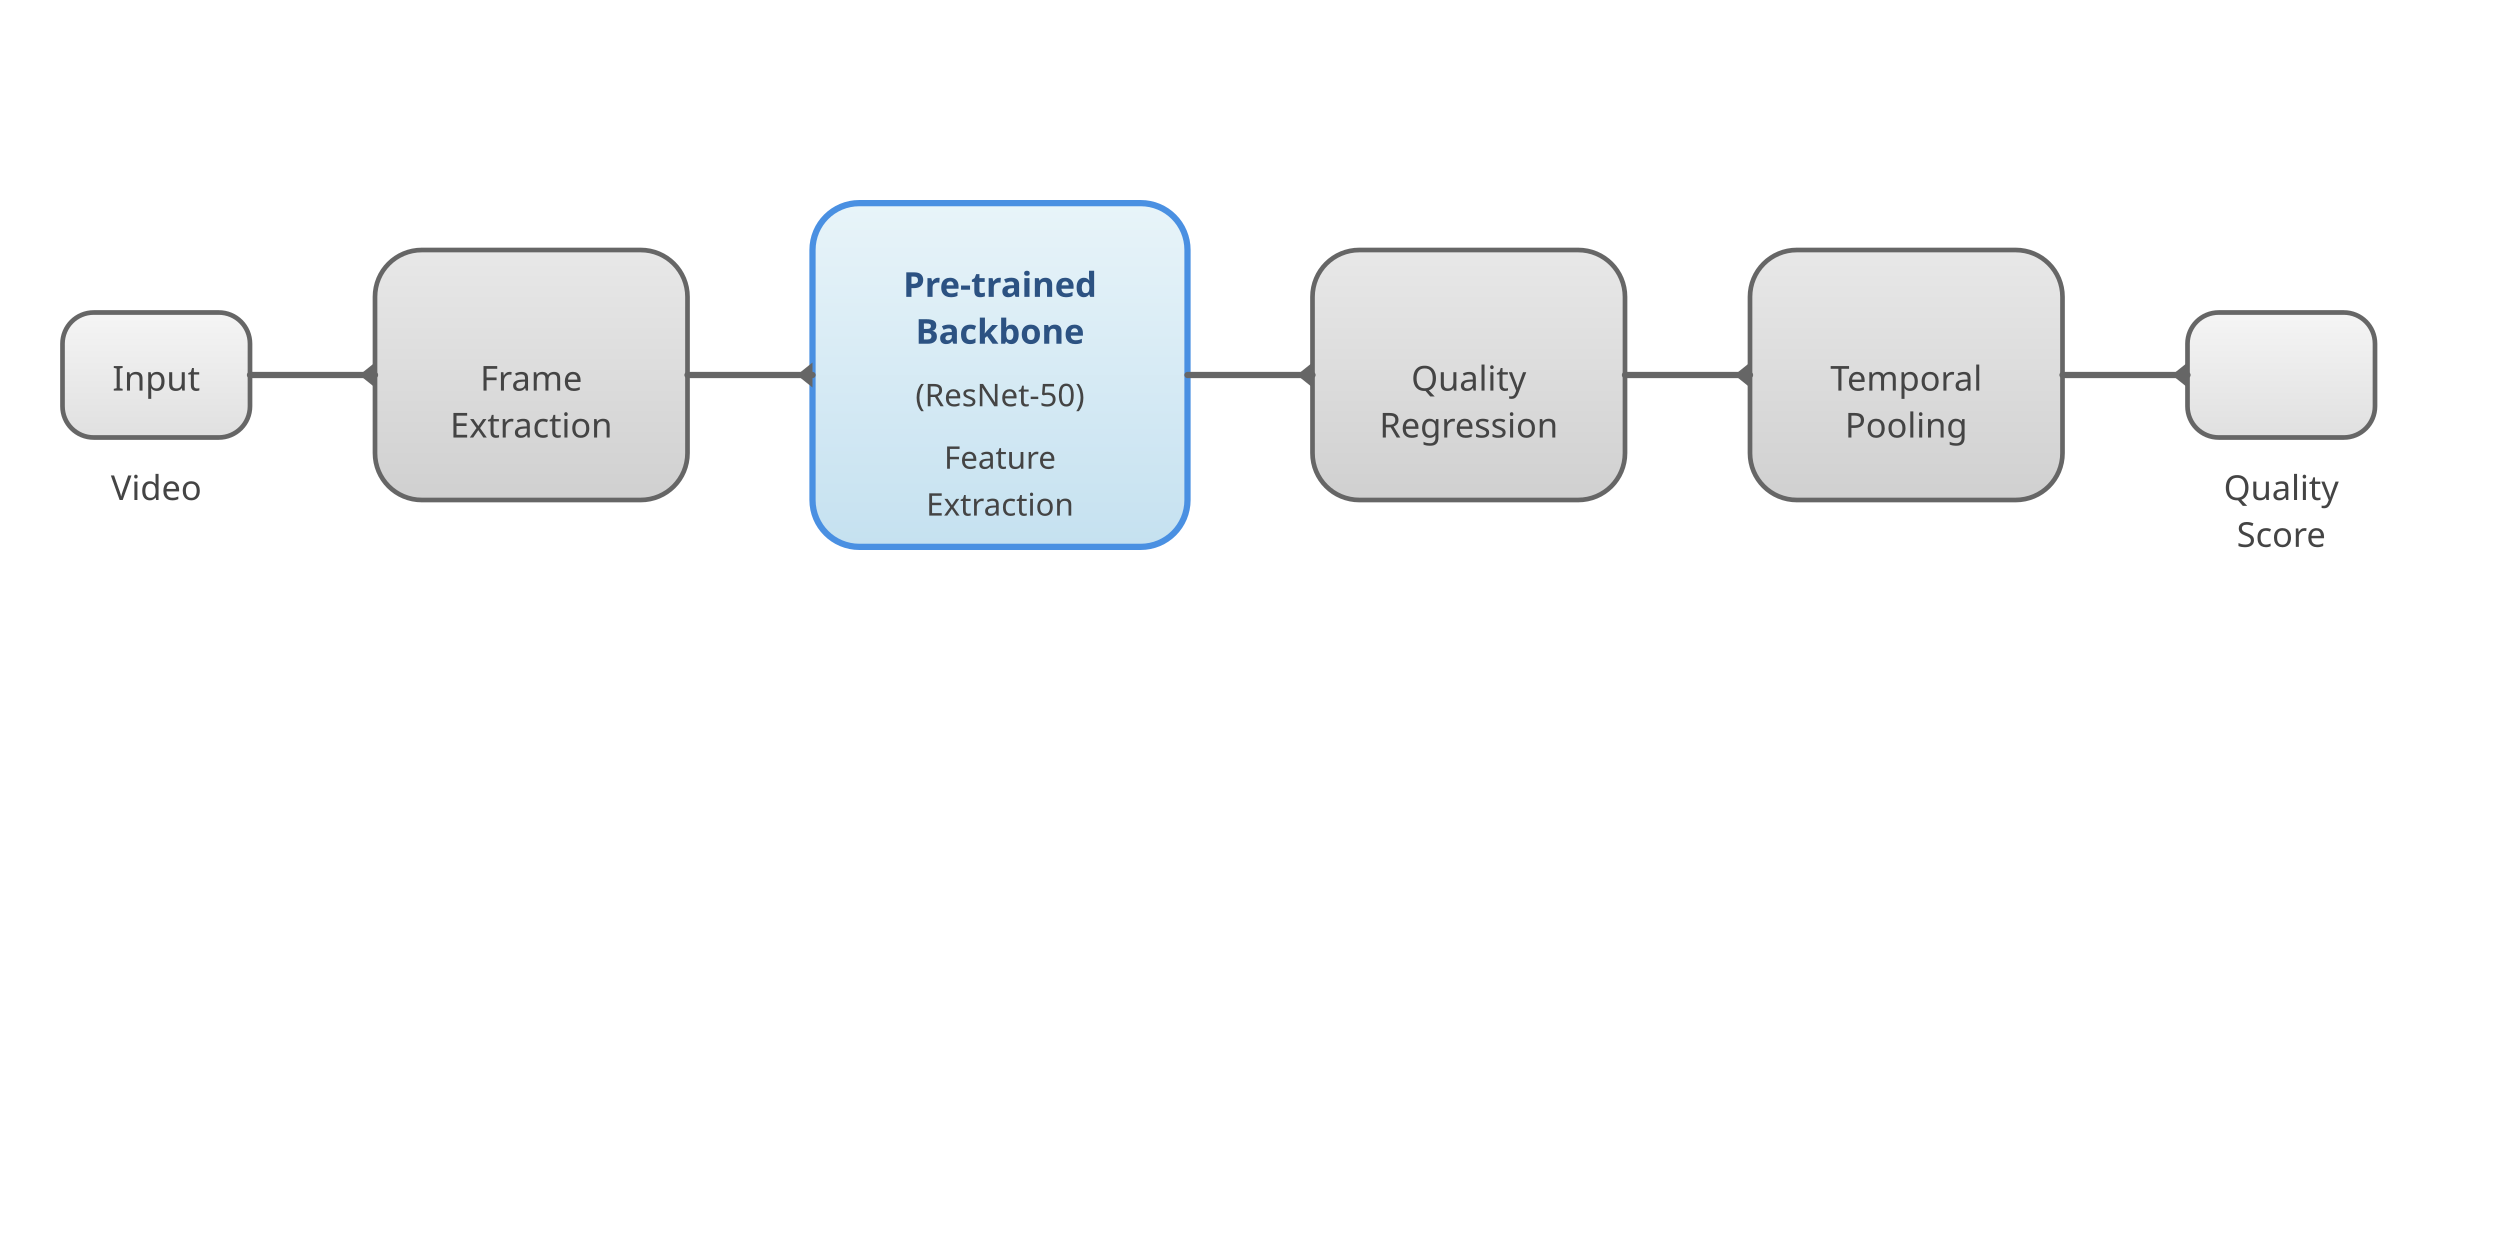
\includegraphics[width=0.9\textwidth]{figures/unified-vqa-framework-3.png}
\caption{Framework of the MDVSFA algorithm proposed by Li, Jiang, and Jiang~\cite{li2023unified}}
\label{fig:framework2}
\end{figure}

The first stage, Relative Quality Assessor, extracts content-aware features from video frames using ResNet-50, followed by temporal integration using a GRU network to model the temporal-memory effect. This stage is supervised by a monotonicity-induced loss, ensuring that the predicted quality ranks are consistent with subjective rankings.

In the second stage, Nonlinear Mapping a four-parameter logistic function is implemented to account for the nonlinearity in human visual perception. This mapping transforms the relative quality scores into perceptual quality scores while maintaining linear correlations with subjective quality, guided by a linearity-induced loss.

Finally, the third stage, Dataset-Specific Perceptual Scale Alignment, addresses inconsistencies in subjective quality score ranges across datasets. A dataset-specific alignment layer maps perceptual quality scores to subjective quality scores specific to each dataset. This alignment is supervised by an error-induced loss, allowing mixed datasets to be utilized effectively during training.

Overall, the MDVSFA framework offers a unified approach to VQA by addressing content dependency, temporal-memory effects, and dataset-specific discrepancies, demonstrating superior performance on multiple in-the-wild datasets~\cite{li2023unified}.

Another high-performing algorithm is the dual-stage attention model proposed by Jia et al.~\cite{jia2024continuous}, specifically designed for continuous and overall Quality of Experience (QoE) evaluation in streaming video. Unlike previous approaches, this model addresses the unique challenges of streaming content, where temporal variations in quality significantly impact user experience. The framework, illustrated in Figure~\ref{fig:framework3}, consists of two primary components: rich feature exploration and dual-stage attention mechanisms.

\begin{figure}
\centering
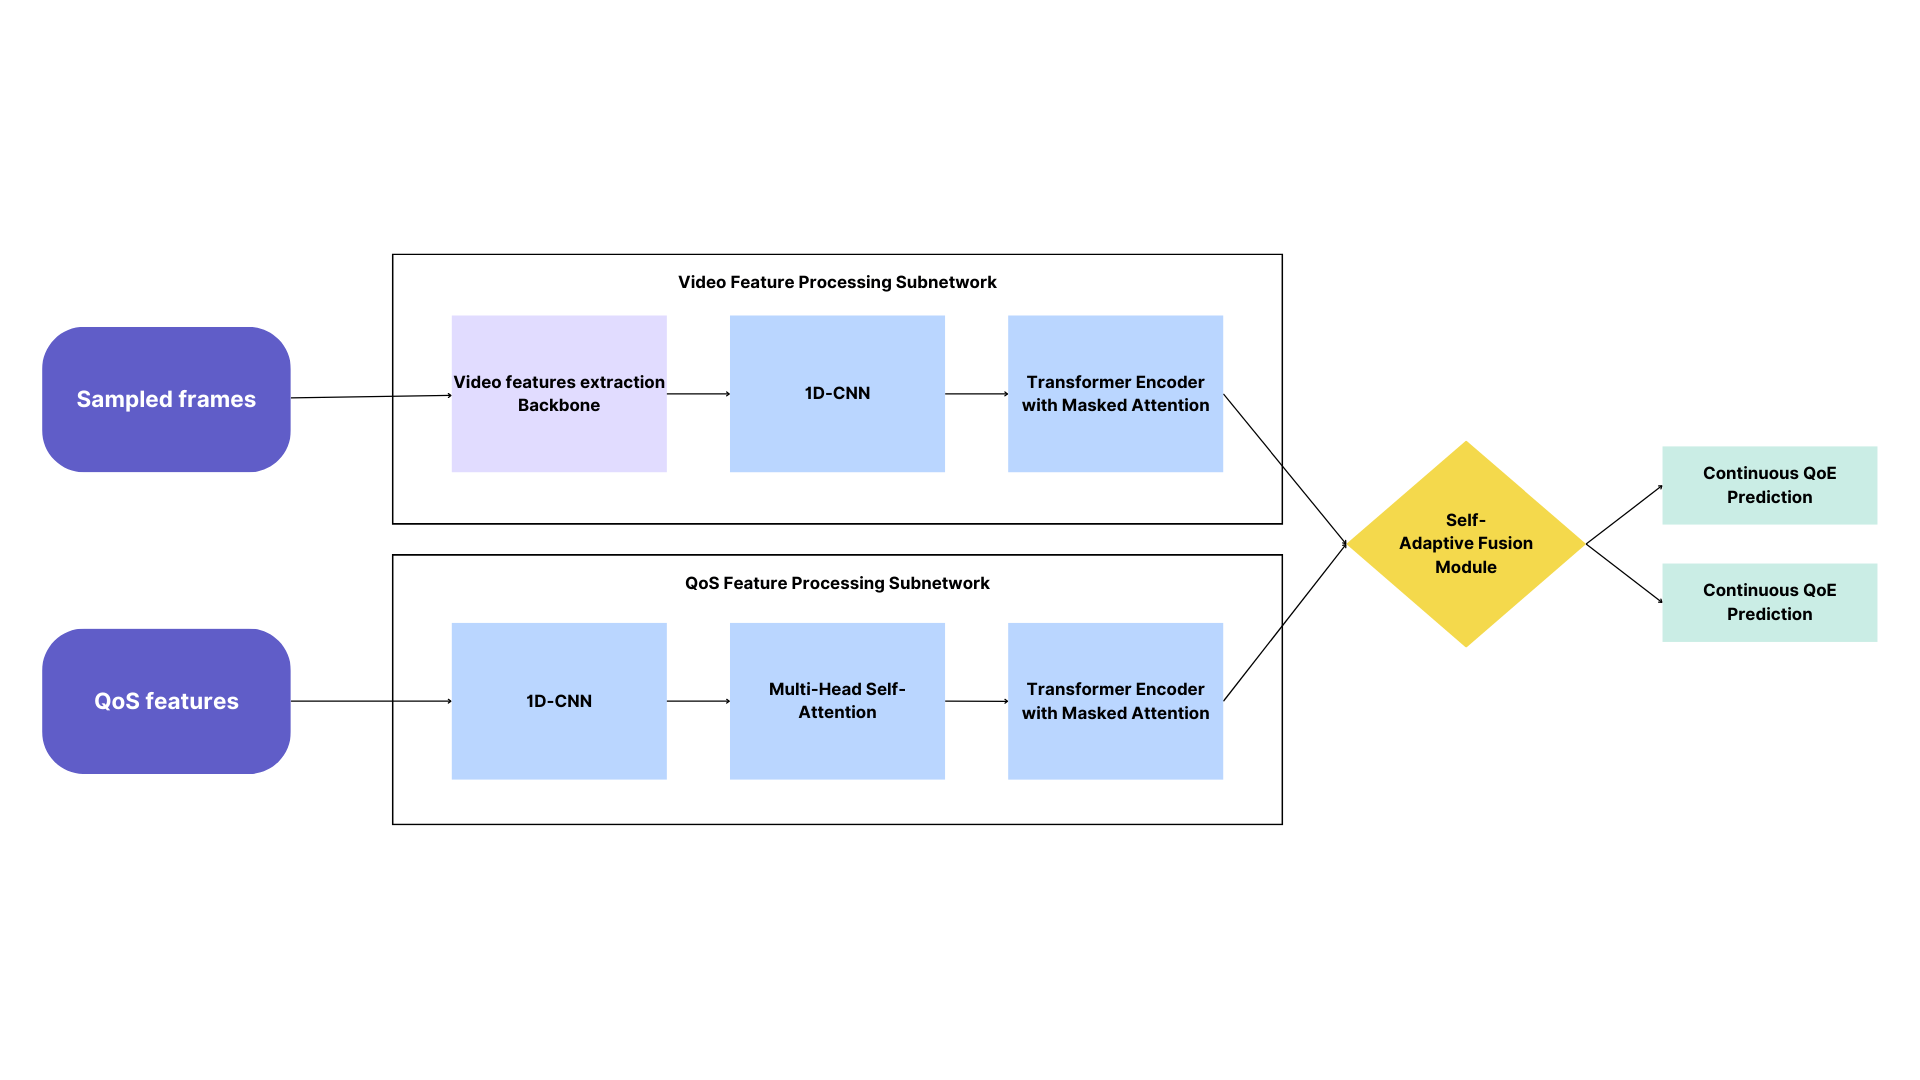
\includegraphics[width=0.9\textwidth]{figures/dual-attention-framework.png}
\caption{Framework of the dual-stage attention model for streaming QoE proposed by Jia et al.~\cite{jia2024continuous}}
\label{fig:framework3}
\end{figure}

To bridge the gap between perceptual video quality and user Quality of Experience (QoE) in streaming scenarios, Jia et al.~\cite{jia2024continuous} propose a unified architecture for both overall and continuous QoE prediction. Their model integrates high-level semantic content features and low-level Quality of Service (QoS) indicators using a dual-stage attention mechanism. 

The architecture comprises two parallel subnetworks: a \textit{video content feature stream} and a \textit{QoS feature stream}. Spatial features are extracted using the final four stages of a pretrained ResNet-50 backbone, while motion features are obtained via the Fast path of a SlowFast network pretrained on Kinetics-400. These are temporally aggregated via global average and standard deviation pooling and concatenated into a 7936-dimensional vector.

The QoS stream encodes time-varying features such as stalling duration, bitrate value, temporal recency of playback disruptions, and bitrate switching dynamics. These features are processed with a grouped 1D-CNN, followed by a \textit{cross-feature attention} (CFA) module based on multi-head self-attention, which captures dependencies among QoS groups and models perceptual non-linearities.

Both feature streams are processed through short-time regression (STR) modules to model short-term quality dynamics, and long-time regression (LTR) modules consisting of Transformer encoder blocks with masked attention to capture long-range temporal dependencies. A \textit{self-adaptive fusion module} then computes a weighted combination of both streams, where the weights are learned as a function of content–QoS interactions. This fusion produces either overall QoE (via temporal pooling and regression) or continuous QoE (frame-level outputs with timestep-wise adaptive fusion).

This model achieves superior performance across multiple public streaming QoE datasets, and its architecture directly reflects key perceptual principles such as content-dependent quality sensitivity and hierarchical processing of temporal and spatial features, making it a strong candidate for real-time QoE inference pipelines.

\section{Algorithms' Performance and Implementation Justification}  
\label{sec:performance_conclusions}

The rapid evolution of adaptive video streaming technologies has necessitated robust methodologies for continuous Quality of Experience (QoE) monitoring. In this work we focus on three state-of-the-art no-reference VQA/QoE frameworks already introduced in Section 2.2: MDVSFA \cite{li2023unified}, FastVQA \cite{wu2022fastvqa}, and the dual-stage attention model \cite{jia2024continuous}. Each model embodies distinct design trade-offs in feature extraction, temporal modeling, and deployment efficiency.

\subsection{Methodological Overview}  
MDVSFA \cite{li2023unified} employs a pretrained ResNet-50 backbone to extract multi-scale spatial features from each frame, integrates temporal context via a GRU, and aligns model outputs to subjective scores through a three-stage pipeline: relative quality ranking (monotonicity loss), nonlinear perceptual mapping (linearity loss), and dataset-specific scale alignment (error-induced loss). This mixed-dataset training yields strong cross-dataset generalization.  

FastVQA \cite{wu2022fastvqa} introduces Grid Mini-patch Sampling (GMS) to fragment each frame into raw-resolution patches, preserving local textures and global structure. A Fragment Attention Network (FANet) built on a hierarchical Swin Transformer processes these fragments, using Gated Relative Position Biases (GRPB) to distinguish intra- vs.\ cross-patch attention, and Intra-Patch Non-Linear Regression (IP-NLR) to avoid feature discontinuity before pooling. FastVQA achieves real-time inference with minimal accuracy loss.  

Dual-Stage Attention \cite{jia2024continuous} unifies continuous and overall QoE prediction by fusing high-level semantic features (ResNet-50 + SlowFast) with low-level QoS indicators (stall duration, bitrate changes, recency). Short-time and long-time temporal regression modules capture local and global temporal dynamics, while a Cross-Feature Attention (CFA) module models perceptual non-linearities among QoS groups. A self-adaptive fusion layer then learns content–QoS weighting for final QoE scores.

\subsection{Comparative Analysis and Selection Rationale}  
MDVSFA's mixed-dataset alignment affords strong cross-dataset performance but relies on frame-level ranking supervision, which can overlook fine-grained temporal artifacts. FastVQA's fragment sampling is codec-agnostic and preserves spatial details, yet its short fragment windows may underrepresent long-term quality drift. The dual-stage attention model explicitly integrates both spatial–temporal features and QoS logs, yielding robust performance across streaming scenarios.  

FastVQA addresses only fragment-level temporal consistency via aligned patch sampling, whereas MDVSFA relies on GRU memory, which can accumulate error over long sequences. Dual-stage attention combines dedicated STR (short-time) and LTR (long-time) modules with masked self-attention, capturing both transient stalls and prolonged bitrate shifts with human-aligned weighting.  

On modern GPU hardware, FastVQA processes 1080p video at over 30 FPS due to its lightweight fragment pipeline. MDVSFA's ResNet-50 + GRU chain runs at 15 FPS for full-resolution frames. The dual-stage attention model incurs higher per-frame cost (20 ms/frame) but remains within real-time budgets when optimized and crucially supports continuous QoE outputs.

Given the need for a unified, codec-agnostic, perceptually accurate and temporally comprehensive QoE predictor—yet still deployable under real-time constraints—we select the dual-stage attention architecture as the centerpiece of this dissertation. Its explicit modeling of both low-level QoS and high-level semantic distortions, combined with dual temporal regression and adaptive fusion, aligns most closely with professional streaming requirements and the goals of this study.  

\section{Neural Networks for Quality-of-Experience Prediction}  
\label{sec:nn_qoe}  

The advent of deep learning has revolutionized Video Quality Assessment (VQA) by enabling data-driven approaches that directly model the complex relationship between video distortions and human perceptual judgments. This section examines neural network architectures specifically engineered for Quality of Experience (QoE) prediction, focusing on their capacity to emulate human visual perception while meeting the computational demands of real-time applications. Unlike generic computer vision models, these architectures incorporate specialized mechanisms to address the unique challenges of perceptual quality assessment, particularly in no-reference scenarios where reference content is unavailable.

\subsection{Architectural Paradigms for Perceptual Quality Prediction}  
Contemporary QoE-driven VQA systems predominantly employ two neural network paradigms, each offering distinct advantages for modeling different aspects of visual quality perception:

\begin{itemize}  
    \item \textbf{Convolutional Neural Networks (CNNs):} These architectures excel at extracting hierarchical spatial features through their localized receptive fields, making them particularly effective at identifying common video artifacts such as blocking, blurring, and banding \cite{he2016deep}. Their inductive biases for translation invariance and local connectivity align well with the Human Visual System's (HVS) early processing stages.
    
    \item \textbf{Vision Transformers (ViTs):} By leveraging self-attention mechanisms, ViTs capture long-range spatiotemporal dependencies that are crucial for modeling global quality perception \cite{dosovitskiy2020image}. Their ability to dynamically weight different regions of the video frame mimics the HVS's attention mechanisms, making them particularly suitable for assessing complex distortions that span multiple spatial and temporal scales.
\end{itemize}  

State-of-the-art implementations typically employ a hybrid approach, where networks are pre-trained on large-scale multimedia datasets (e.g., ImageNet, Kinetics) and subsequently fine-tuned for VQA-specific tasks \cite{li2023unified}. This transfer learning paradigm enables robust feature representation while mitigating the data scarcity challenges inherent to perceptual quality assessment.

\subsection{Case Study: Hierarchical Feature Extraction with ResNet-50}  
The framework proposed by Li \textit{et al.}~\cite{li2023unified} serves as an exemplary implementation of CNN-based QoE prediction, demonstrating how traditional computer vision architectures can be adapted for perceptual quality assessment. The system employs a two-stage processing pipeline that addresses both low-level distortion detection and high-level quality estimation:

\begin{enumerate}  
    \item \textbf{Multi-Scale Spatiotemporal Feature Extraction:}  
    \begin{itemize}  
        \item The ResNet-50 backbone processes individual video frames through its convolutional layers, generating a hierarchy of feature maps that capture distortions at varying spatial scales (from pixel-level artifacts to frame-wide impairments).
        \item Temporal dynamics are modeled through a combination of 3D convolutions and recurrent units (GRUs), which aggregate features across successive frames to account for motion-related distortions and temporal masking effects \cite{lee2021video}.
    \end{itemize}  
    
    \item \textbf{Feature Normalization and Quality Regression:}  
    \begin{itemize}  
        \item Domain-specific normalization techniques (e.g., instance normalization with learned parameters) are applied to mitigate dataset biases arising from varying resolutions, bitrates, and content types.
        \item Spatial average pooling generates compact, content-agnostic feature descriptors that feed into a quality regression head, which predicts MOS scores through fully connected layers.
    \end{itemize}  
\end{enumerate}  

This architecture demonstrates how traditional CNN designs can be effectively repurposed for perceptual quality assessment by incorporating temporal modeling and domain adaptation components.

\subsection{Optimizing for Perceptual Alignment}  
Achieving accurate quality prediction requires careful alignment between computational models and human perceptual mechanisms. Modern QoE-driven VQA systems address this through two principal strategies: advanced loss function design and biologically-inspired attention mechanisms.

The design of perceptually-weighted loss functions extends beyond conventional mean squared error (MSE) optimization. Recent work by \cite{min2024perceptual} demonstrates that incorporating temporal weighting factors accounts for the recency effect in human quality judgments, where viewers tend to disproportionately weight the quality of recent video segments. Additionally, content-adaptive weighting schemes emphasize distortion visibility in perceptually critical regions, such as areas with high spatial frequency content or salient objects, while reducing emphasis on less visually important regions. These approaches mirror findings from psychovisual studies showing that human quality perception is non-uniform across both spatial and temporal dimensions.

Attention mechanisms play a particularly crucial role in bridging the gap between artificial quality assessment and human perception. As demonstrated by \cite{wu2022fastvqa}, spatial and channel attention modules dynamically modulate feature importance based on distortion visibility, effectively mimicking the Human Visual System's (HVS) selective attention processes. Neuropsychological research has shown that the HVS employs similar mechanisms to prioritize processing of visually salient regions while suppressing less relevant information \cite{itti1998model}. In VQA systems, this manifests as learned attention patterns that emphasize:
\begin{itemize}
    \item Texture-rich regions where compression artifacts are most visible
    \item Motion boundaries affected by temporal compression
    \item High-contrast edges susceptible to ringing artifacts
\end{itemize}
This biological plausibility contributes to the models' ability to predict subjective quality judgments with high accuracy, as evidenced by their strong correlation with Mean Opinion Scores (MOS) across diverse content types and distortion profiles. 

\subsection{Implementation Challenges and Practical Considerations}  
Despite their demonstrated effectiveness, neural network-based QoE predictors face several persistent challenges that influence architectural choices and deployment strategies:

\begin{itemize}  
    \item \textbf{Data Scarcity and Annotation Costs:} The labor-intensive nature of subjective quality assessment severely limits dataset sizes, with most public benchmarks containing fewer than 1,000 annotated sequences \cite{hosu2020konvid}. This scarcity is compounded by the domain gap between different datasets, as noted by \cite{li2023unified}. Recent approaches address these limitations through several strategies: robust cross-dataset training frameworks that learn domain-invariant features, semi-supervised techniques leveraging unlabeled data, and synthetic data generation methods that preserve perceptual quality relationships. The MDVSFA architecture \cite{li2023unified} demonstrates particular effectiveness in cross-dataset scenarios through its unified quality assessment paradigm.
    
    \item \textbf{Computational Complexity:} Vision Transformers (ViTs) achieve state-of-the-art performance but require significant computational resources due to their quadratic complexity with respect to input size \cite{liu2021swin}. Their deployment typically necessitates powerful GPU hardware, though recent advances in model compression techniques have improved their practicality. Quantization methods, for instance, can reduce model size and computation requirements by using lower-precision arithmetic without significant quality prediction degradation. Efficient attention variants like shifted window approaches and hybrid CNN-Transformer architectures offer additional pathways for balancing accuracy and computational demands.
    
    \item \textbf{Interpretability and Explainability:} The black-box nature of deep quality predictors complicates their adoption in production environments. While techniques like Grad-CAM \cite{selvaraju2017grad} provide post-hoc explanations by visualizing spatial contributions to quality predictions, more intrinsic interpretability remains an open research challenge. This is particularly crucial for applications requiring quality-based decision making, where stakeholders need to understand the rationale behind quality scores.
\end{itemize}  

\section{Rust and Machine Learning Inference in Media Pipelines}

Although most machine learning (ML) inference pipelines are traditionally implemented in high-level languages such as Python or in low-level C/C++ stacks, the Rust programming language has emerged as a promising alternative for system-level deployment of real-time media and AI applications. Rust's emphasis on safety, concurrency, and performance makes it a suitable candidate for time-sensitive, memory-safe environments like media streaming infrastructures.

One important development in this direction is the growing use of \textbf{GStreamer}, an open-source multimedia pipeline framework that has become a standard in many Linux-based distributions and platforms. As noted in Ham et al.~\cite{ham2019nnstreamer}, ``GStreamer~\cite{gstreamer1999} is the standard multimedia pipeline framework for Tizen and many Linux distributions. GStreamer provides APIs and utilities to construct stream pipelines for multimedia applications of various platforms including Linux, Android, Windows, iOS, and macOS. GStreamer is highly modular; every filter and path control is implemented as a plugin attached in run-time. GStreamer has been applied to various systems where multimedia performance matters. BBC uses GStreamer for their broadcasting system.''

In particular, the NNStreamer project~\cite{ham2019nnstreamer} extends GStreamer to integrate neural network inference directly into the media pipeline by treating trained ML models as stream filters. This approach streamlines the execution of deep learning models on-device and serves as an important precedent for real-time AI-augmented media processing.

While GStreamer has traditionally relied on C and C++, recent developments have demonstrated the feasibility of integrating Rust into these pipelines. The modularity and runtime plugin architecture of GStreamer make it particularly conducive to Rust-based components, providing the opportunity for safer and more reliable media applications.

Despite Rust's increasing popularity, gaps remain in the academic and industrial literature regarding its use in real-time ML inference for media pipelines. As noted by Beltrán-Escobar et al.~\cite{beltran2024review}, Rust's adoption in embedded systems and computer vision has accelerated in recent years, especially within the TinyML community. However, they emphasize that “no low- or large-scale commercial and industrial applications using Rust language for real-time image processing and control systems have been reported.” This underscores the need for empirical studies and practical implementations that explore Rust's capabilities in this domain.

Further, a recent systematic survey by Sharma et al.~\cite{sharma2023rust} highlights both the promise and the challenges of using Rust in embedded environments. Their findings suggest that while Rust addresses many traditional safety pitfalls in C-based embedded systems, its ecosystem maturity and integration with advanced ML toolchains are still evolving.

In light of this context, this dissertation offers a novel contribution by implementing a state-of-the-art neural network model for no-reference video quality assessment (NR-VQA) in a Rust-based media pipeline. It serves as an exploratory trial to bridge the gap between research and deployment, extending the practical knowledge base for using Rust in AI-augmented multimedia systems, with relevance for both embedded and cloud-scale scenarios.

\section{Synthesis and Architectural Innovations}

Several recent deep VQA/QoE models have pushed the state-of-the-art while highlighting different design trade‑offs. \textbf{FAST-VQA} (Wu \textit{et al.}, 2022) uses a grid-based ``fragment'' sampling of raw-resolution patches and a dedicated fragment-attention transformer (FANet) to capture local and global quality cues. This end-to-end model achieves $\approx$10\% accuracy gains over prior VQA methods while dramatically reducing compute for high-resolution videos~\cite{wu2022fastvqa}. \textbf{MDTVSFA} (Li \textit{et al.}, 2021) addresses the cross-dataset problem by training a single model on mixed VQA datasets. It explicitly models human perception (content dependency and temporal memory) and includes stages of relative quality assessment, nonlinear mapping, and dataset-specific perceptual scale alignment~\cite{li2023unified}. This unified approach demonstrated superior cross-dataset performance compared to specialized models~\cite{li2023unified}. In contrast, some streaming-QoE models (e.g. \textit{DA-QoE}) combine hand-crafted QoS and visual features with recurrent networks to predict QoE scores, but often rely on explicit network or compression statistics and lack deep perceptual modeling~\cite{li2022weakly}.

Most of these advances focus on off-line VQA accuracy on standard datasets, and few explicitly target the constraints of real-time content distribution. For example, Bampis and Bovik observe that conventional VQA metrics fail to predict human QoE when streaming impairments like rebuffering and bitrate changes occur~\cite{BAMPIS2018218}. In practice, live streaming requires low-latency, high-reliability assessments that account for temporal attention and episodic events (e.g. stalls), which many models do not handle. FAST-VQA and MDTVSFA are powerful but primarily designed for static evaluation rather than continuous playback scenarios. Likewise, models like DA-QoE or GCNN-QoE use statistical features and GRUs, which may not fully capture perceptual nuance or may introduce latency in inference.

The \textbf{dual-stage attention} approach of Jia \textit{et al.} (2024) bridges these gaps. Their DSA-QoE network explicitly models temporal attention and cross-feature attention to predict \textit{continuous} QoE alongside overall scores~\cite{jia2024continuous}. In experiments on multiple streaming QoE datasets, this model significantly outperforms prior methods, underscoring the value of human-like attention mechanisms in QoE prediction. Because it is a no-reference, codec-agnostic model focused on perceptual quality, it is well-suited to real-world streaming content.

Over the past decade, deep learning–based no-reference video quality assessment (NR-VQA) and Quality of Experience (QoE) models have achieved remarkable progress by leveraging increasingly sophisticated feature extraction and temporal modeling techniques. The FastVQA framework introduced by Wu \textit{et al.}~\cite{wu2022fastvqa} exemplifies an efficiency-oriented design: by fragmenting each frame into raw-resolution patches via Grid Mini-patch Sampling (GMS) and processing these through a hierarchical Swin Transformer–based Fragment Attention Network (FANet), FastVQA attains a nearly 10\% improvement in Spearman's rank correlation over prior methods while sustaining real-time throughput for high-resolution video input. However, despite its compelling balance of spatial fidelity and computational efficiency, FastVQA's short-window fragment sampling is not explicitly attuned to the episodic temporal distortions—such as rebuffering stalls and bitrate variations—that critically shape viewer experience in live streaming applications.

In contrast, the MDVSFA model proposed by Li \textit{et al.}~\cite{li2023unified} addresses the challenge of cross-dataset generalization through a unified, mixed-dataset training strategy. MDVSFA employs a pretrained ResNet-50 backbone to extract multi-scale spatial feature maps and integrates temporal context via a Gated Recurrent Unit (GRU). Its three-stage supervision—comprising relative quality ranking (monotonicity loss), nonlinear perceptual mapping (linearity loss), and dataset-specific scale alignment (error-induced loss)—enables the model to produce MOS predictions that remain well-calibrated across diverse video domains. Nevertheless, the reliance on GRU-based temporal aggregation can lead to drift when modeling long-duration sequences, and the absence of explicit mechanisms for modeling low-level playback metrics limits its sensitivity to critical streaming impairments.

The dual-stage attention architecture of Jia \textit{et al.}~\cite{jia2024continuous} synthesizes the strengths of both high-level content modeling and low-level QoS feature integration within a unified framework tailored for continuous and overall QoE prediction. In this scheme, semantic features are extracted from the final four stages of a ResNet-50 backbone and from the fast pathway of a SlowFast network pretrained on Kinetics-400, while QoS features—including stalling indicators, bitrate representations, temporal recency, and bitrate switch dynamics—are processed through grouped 1D-CNNs to preserve feature-wise granularity. Short-time and long-time temporal regression modules, respectively implemented via masked 1D convolutions and Transformer-based masked self-attention, capture both immediate and protracted temporal dependencies. A cross-feature attention (CFA) module further models the perceptual non-linearities among QoS feature groups, and a self-adaptive fusion mechanism learns content–QoS weighting to produce final QoE scores. Empirical evaluations demonstrate that this model attains Spearman's rank correlations up to 0.89 on live streaming datasets, outperforming both FastVQA and MDVSFA in capturing real-world streaming anomalies.

In summary, while FastVQA~\cite{wu2022fastvqa} and MDVSFA~\cite{li2023unified} have advanced the frontiers of efficient spatial–temporal feature extraction and cross-dataset robustness, respectively, they lack dedicated mechanisms for jointly modeling network-induced impairments and perceptual feature fusion over varying temporal scales. Conversely, the dual-stage attention model~\cite{jia2024continuous} provides a comprehensive solution by integrating semantic and QoS streams through hierarchical attention and adaptive fusion, thereby reconciling the demands of low-latency inference, perceptual fidelity, and codec-agnostic deployment. These characteristics render it the most suitable foundation for real-time QoE monitoring in professional audiovisual distribution pipelines.

Jia et al.'s dual-stage attention architecture emerges as the most viable solution, harmonizing accuracy, efficiency, and adaptability. Its ability to localize distortion-prone regions via attention maps not only enhances interpretability but also aligns with human visual saliency, making it uniquely suited for deployment in dynamic, multi-codec streaming platforms. The selection of this model is further vindicated by its modular design, which facilitates seamless integration into existing media pipelines without requiring architectural overhauls—a critical consideration for industry adoption.

To complement this architectural innovation, the implementation of this model within a Rust-based media pipeline represents a novel contribution to the systems-level deployment of real-time QoE solutions. Rust's strong guarantees of memory and concurrency safety, zero-cost abstractions, and absence of garbage collection provide the necessary foundations for high-performance streaming applications~\cite{fulton2022benefits}. Its integration within modular frameworks such as GStreamer has been increasingly explored, and its feasibility for embedded machine learning inference has been demonstrated by projects like MicroFlow~\cite{carnelos2025microflow}. Despite its growing academic presence, recent reviews~\cite{beltran2024review,sharma2023rust} point out a lack of reported large-scale deployments in real-time media processing systems. By embedding DSA-QoE within a Rust-powered inference pipeline, this dissertation not only tests the architectural strengths of dual-stage attention but also addresses a gap in the literature regarding the operational viability of Rust for AI-augmented multimedia applications.